\chapter{Combinatoria}

\index{combinatoria}

\key{Combinatoria} estudia métodos para contar combinaciones de objetos.
Usualmente, el objetivo es encontrar una manera de
contar las combinaciones de manera eficiente
sin generar cada combinación por separado.

Como ejemplo, considere el problema
de contar la cantidad de formas de
representar un entero $n$ como una suma de enteros positivos.
Por ejemplo, hay 8 representaciones
para $4$:
\begin{multicols}{2}
\begin{itemize}
\item $1+1+1+1$
\item $1+1+2$
\item $1+2+1$
\item $2+1+1$
\item $2+2$
\item $3+1$
\item $1+3$
\item $4$
\end{itemize}
\end{multicols}

Un problema combinatorio a menudo se puede resolver
usando una función recursiva.
En este problema, podemos definir una función $f(n)$
que da la cantidad de representaciones para $n$.
Por ejemplo, $f(4)=8$ de acuerdo con el ejemplo anterior.
Los valores de la función
se pueden calcular recursivamente de la siguiente manera:
\begin{equation*}
    f(n) = \begin{cases}
               1               & n = 0\\
               f(0)+f(1)+\cdots+f(n-1) & n > 0\\
           \end{cases}
\end{equation*}
El caso base es $f(0)=1$,
porque la suma vacía representa el número 0.
Entonces, si $n>0$, consideramos todas las formas de
elegir el primer número de la suma.
Si el primer número es $k$,
hay $f(n-k)$ representaciones
para la parte restante de la suma.
Por lo tanto, calculamos la suma de todos los valores
de la forma $f(n-k)$ donde $k<n$.

Los primeros valores para la función son:
\[
\begin{array}{lcl}
f(0) & = & 1 \\
f(1) & = & 1 \\
f(2) & = & 2 \\
f(3) & = & 4 \\
f(4) & = & 8 \\
\end{array}
\]

A veces, una fórmula recursiva se puede reemplazar
con una fórmula de forma cerrada.
En este problema,
\[
f(n)=2^{n-1},
\]
que se basa en el hecho de que hay $n-1$
posiciones posibles para los signos +- en la suma
y podemos elegir cualquier subconjunto de ellos.

\section{Coeficientes binomiales}

\index{coeficiente binomial}

El \key{coeficiente binomial} ${n \choose k}$
es igual al número de formas en que podemos elegir un subconjunto
de $k$ elementos de un conjunto de $n$ elementos.
Por ejemplo, ${5 \choose 3}=10$,
porque el conjunto $\{1,2,3,4,5\}$
tiene 10 subconjuntos de 3 elementos:
\[ \{1,2,3\}, \{1,2,4\}, \{1,2,5\}, \{1,3,4\}, \{1,3,5\}, 
\{1,4,5\}, \{2,3,4\}, \{2,3,5\}, \{2,4,5\}, \{3,4,5\} \]

\subsubsection{Fórmula 1}

Los coeficientes binomiales se pueden
calcular recursivamente de la siguiente manera:

\[
{n \choose k}  =  {n-1 \choose k-1} + {n-1 \choose k}
\]

La idea es fijar un elemento $x$ en el conjunto.
Si $x$ está incluido en el subconjunto,
tenemos que elegir $k-1$
elementos de $n-1$ elementos,
y si $x$ no está incluido en el subconjunto,
tenemos que elegir $k$ elementos de $n-1$ elementos.

Los casos base para la recursión son
\[
{n \choose 0}  =  {n \choose n} = 1,
\]
porque siempre hay exactamente
una forma de construir un subconjunto vacío
y un subconjunto que contiene todos los elementos.

\subsubsection{Fórmula 2}

Otra forma de calcular los coeficientes binomiales es la siguiente:
\[
{n \choose k}  =  \frac{n!}{k!(n-k)!}.
\]

Hay $n!$ permutaciones de $n$ elementos.
Recorremos todas las permutaciones y siempre
incluimos los primeros $k$ elementos de la permutación
en el subconjunto.
Dado que el orden de los elementos en el subconjunto
y fuera del subconjunto no importa,
el resultado se divide por $k!$ y $(n-k)!$

\subsubsection{Propiedades}

Para los coeficientes binomiales,
\[
{n \choose k}  =  {n \choose n-k},
\]
porque en realidad dividimos un conjunto de $n$ elementos en
dos subconjuntos: el primero contiene $k$ elementos
y el segundo contiene $n-k$ elementos.

La suma de los coeficientes binomiales es
\[
{n \choose 0}+{n \choose 1}+{n \choose 2}+\ldots+{n \choose n}=2^n.
\]

La razón del nombre ''coeficiente binomial''
se puede ver cuando el binomio $(a+b)$ se eleva a
la $n$ésima potencia:

\[ (a+b)^n =
{n \choose 0} a^n b^0 + 
{n \choose 1} a^{n-1} b^1 +
\ldots + 
{n \choose n-1} a^1 b^{n-1} +
{n \choose n} a^0 b^n. \]

\index{Triángulo de Pascal}

Los coeficientes binomiales también aparecen en
el \key{Triángulo de Pascal}
donde cada valor es igual a la suma de dos
valores arriba:
\begin{center}
\begin{tikzpicture}{0.9}
\node at (0,0) {1};
\node at (-0.5,-0.5) {1};
\node at (0.5,-0.5) {1};
\node at (-1,-1) {1};
\node at (0,-1) {2};
\node at (1,-1) {1};
\node at (-1.5,-1.5) {1};
\node at (-0.5,-1.5) {3};
\node at (0.5,-1.5) {3};
\node at (1.5,-1.5) {1};
\node at (-2,-2) {1};
\node at (-1,-2) {4};
\node at (0,-2) {6};
\node at (1,-2) {4};
\node at (2,-2) {1};
\node at (-2,-2.5) {$\ldots$};
\node at (-1,-2.5) {$\ldots$};
\node at (0,-2.5) {$\ldots$};
\node at (1,-2.5) {$\ldots$};
\node at (2,-2.5) {$\ldots$};
\end{tikzpicture}
\end{center}

\subsubsection{Cajas y bolas}

''Cajas y bolas'' es un modelo útil,
donde contamos las formas de
colocar $k$ bolas en $n$ cajas.
Consideremos tres escenarios:

\textit{Escenario 1}: Cada caja puede contener
como máximo una bola.
Por ejemplo, cuando $n=5$ y $k=2$,
hay 10 soluciones:

\begin{center}
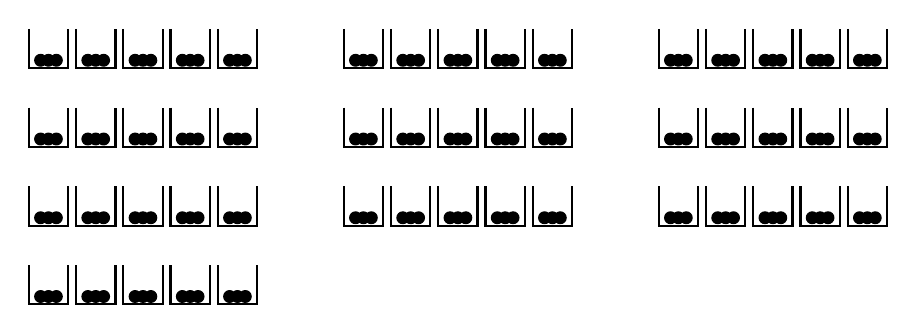
\begin{tikzpicture}[scale=0.5]
\newcommand\lax[3]{
\path[draw,thick,-] (#1-0.5,#2+0.5) -- (#1-0.5,#2-0.5) --
                    (#1+0.5,#2-0.5) -- (#1+0.5,#2+0.5);
\ifthenelse{\equal{#3}{1}}{\draw[fill=black] (#1,#2-0.3) circle (0.15);}{}
\ifthenelse{\equal{#3}{2}}{\draw[fill=black] (#1-0.2,#2-0.3) circle (0.15);}{}
\ifthenelse{\equal{#3}{2}}{\draw[fill=black] (#1+0.2,#2-0.3) circle (0.15);}{}
}
\newcommand\laa[7]{
    \lax{#1}{#2}{#3}
    \lax{#1+1.2}{#2}{#4}
    \lax{#1+2.4}{#2}{#5}
    \lax{#1+3.6}{#2}{#6}
    \lax{#1+4.8}{#2}{#7}
}

\laa{0}{0}{1}{1}{0}{0}{0}
\laa{0}{-2}{1}{0}{1}{0}{0}
\laa{0}{-4}{1}{0}{0}{1}{0}
\laa{0}{-6}{1}{0}{0}{0}{1}
\laa{8}{0}{0}{1}{1}{0}{0}
\laa{8}{-2}{0}{1}{0}{1}{0}
\laa{8}{-4}{0}{1}{0}{0}{1}
\laa{16}{0}{0}{0}{1}{1}{0}
\laa{16}{-2}{0}{0}{1}{0}{1}
\laa{16}{-4}{0}{0}{0}{1}{1}

\end{tikzpicture}
\end{center}

En este escenario, la respuesta es directamente el
coeficiente binomial ${n \choose k}$.

\textit{Escenario 2}: Una caja puede contener múltiples bolas.
Por ejemplo, cuando $n=5$ y $k=2$,
hay 15 soluciones:

\begin{center}
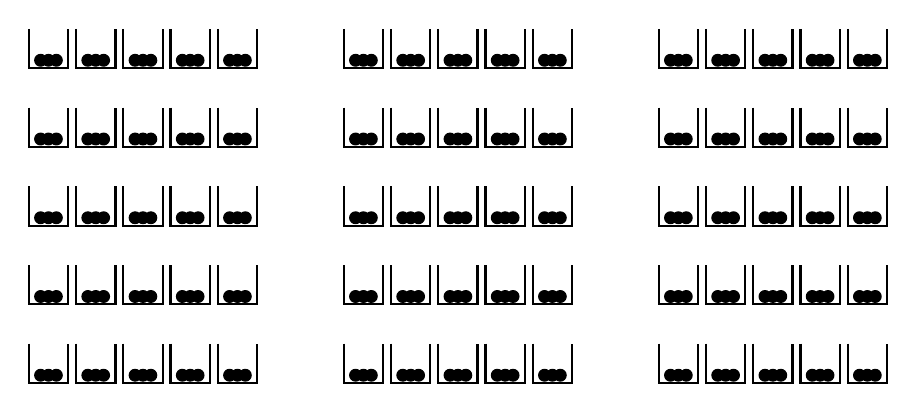
\begin{tikzpicture}[scale=0.5]
\newcommand\lax[3]{
\path[draw,thick,-] (#1-0.5,#2+0.5) -- (#1-0.5,#2-0.5) --
                    (#1+0.5,#2-0.5) -- (#1+0.5,#2+0.5);
\ifthenelse{\equal{#3}{1}}{\draw[fill=black] (#1,#2-0.3) circle (0.15);}{}
\ifthenelse{\equal{#3}{2}}{\draw[fill=black] (#1-0.2,#2-0.3) circle (0.15);}{}
\ifthenelse{\equal{#3}{2}}{\draw[fill=black] (#1+0.2,#2-0.3) circle (0.15);}{}
}
\newcommand\laa[7]{
    \lax{#1}{#2}{#3}
    \lax{#1+1.2}{#2}{#4}
    \lax{#1+2.4}{#2}{#5}
    \lax{#1+3.6}{#2}{#6}
    \lax{#1+4.8}{#2}{#7}
}

\laa{0}{0}{2}{0}{0}{0}{0}
\laa{0}{-2}{1}{1}{0}{0}{0}
\laa{0}{-4}{1}{0}{1}{0}{0}
\laa{0}{-6}{1}{0}{0}{1}{0}
\laa{0}{-8}{1}{0}{0}{0}{1}
\laa{8}{0}{0}{2}{0}{0}{0}
\laa{8}{-2}{0}{1}{1}{0}{0}
\laa{8}{-4}{0}{1}{0}{1}{0}
\laa{8}{-6}{0}{1}{0}{0}{1}
\laa{8}{-8}{0}{0}{2}{0}{0}
\laa{16}{0}{0}{0}{1}{1}{0}
\laa{16}{-2}{0}{0}{1}{0}{1}
\laa{16}{-4}{0}{0}{0}{2}{0}
\laa{16}{-6}{0}{0}{0}{1}{1}
\laa{16}{-8}{0}{0}{0}{0}{2}

\end{tikzpicture}
\end{center}

El proceso de colocar las bolas en las cajas
puede ser representado como una cadena
que consiste en símbolos
''o'' y ''$\rightarrow$''.
Inicialmente, asumamos que estamos parados en la caja más a la izquierda.
El símbolo ''o'' significa que colocamos una bola
en la caja actual, y el símbolo
''$\rightarrow$'' significa que nos movemos a
la siguiente caja a la derecha.

Usando esta notación, cada solución es una cadena
que contiene $k$ veces el símbolo ''o'' y
$n-1$ veces el símbolo ''$\rightarrow$''.
Por ejemplo, la solución de arriba a la derecha
en la imagen anterior corresponde a la cadena
''$\rightarrow$ $\rightarrow$ o $\rightarrow$ o $\rightarrow$''.
Así, el número de soluciones es
${k+n-1 \choose k}$.

\textit{Escenario 3}: Cada caja puede contener como máximo una bola,
y además, ninguna de las dos cajas adyacentes puede contener una bola.
Por ejemplo, cuando $n=5$ y $k=2$,
hay 6 soluciones:


\begin{center}
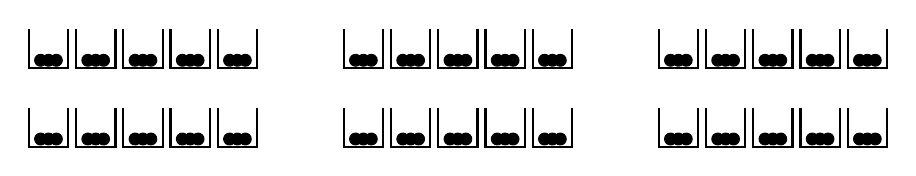
\begin{tikzpicture}[scale=0.5]
\newcommand\lax[3]{
\path[draw,thick,-] (#1-0.5,#2+0.5) -- (#1-0.5,#2-0.5) --
                    (#1+0.5,#2-0.5) -- (#1+0.5,#2+0.5);
\ifthenelse{\equal{#3}{1}}{\draw[fill=black] (#1,#2-0.3) circle (0.15);}{}
\ifthenelse{\equal{#3}{2}}{\draw[fill=black] (#1-0.2,#2-0.3) circle (0.15);}{}
\ifthenelse{\equal{#3}{2}}{\draw[fill=black] (#1+0.2,#2-0.3) circle (0.15);}{}
}
\newcommand\laa[7]{
    \lax{#1}{#2}{#3}
    \lax{#1+1.2}{#2}{#4}
    \lax{#1+2.4}{#2}{#5}
    \lax{#1+3.6}{#2}{#6}
    \lax{#1+4.8}{#2}{#7}
}

\laa{0}{0}{1}{0}{1}{0}{0}
\laa{0}{-2}{1}{0}{0}{1}{0}
\laa{8}{0}{1}{0}{0}{0}{1}
\laa{8}{-2}{0}{1}{0}{1}{0}
\laa{16}{0}{0}{1}{0}{0}{1}
\laa{16}{-2}{0}{0}{1}{0}{1}
\end{tikzpicture}
\end{center}

En este escenario, podemos asumir que
$k$ bolas se colocan inicialmente en las cajas
y hay una caja vacía entre cada
dos cajas adyacentes.
La tarea restante es elegir
las posiciones para las cajas vacías restantes.
Hay $n-2k+1$ cajas de este tipo y
$k+1$ posiciones para ellas.
Así, usando la fórmula del escenario 2,
el número de soluciones es
${n-k+1 \choose n-2k+1}$.

\subsubsection{Coeficientes multinomiales}

\index{coeficiente multinomial}

El \key{coeficiente multinomial}
\[ {n \choose k_1,k_2,\ldots,k_m} = \frac{n!}{k_1! k_2! \cdots k_m!}, \]
es igual al número de maneras
en que podemos dividir $n$ elementos en subconjuntos
de tamaños $k_1,k_2,\ldots,k_m$,
donde $k_1+k_2+\cdots+k_m=n$.
Los coeficientes multinomiales pueden verse como una
generalización de los coeficientes binomiales;
si $m=2$, la fórmula anterior
corresponde a la fórmula del coeficiente binomial.

\section{Números de Catalan}

\index{número de Catalan}

El \key{número de Catalan}
%\footnote{E. C. Catalan (1814--1894) fue un matemático belga.}
$C_n$ es igual al
número de expresiones de paréntesis válidas que consisten en
$n$ paréntesis izquierdos y $n$ paréntesis derechos.

Por ejemplo, $C_3=5$, porque
podemos construir las siguientes expresiones de paréntesis
usando tres
paréntesis izquierdos y derechos:



\begin{itemize}[noitemsep]
\item \texttt{()()()}
\item \texttt{(())()}
\item \texttt{()(())}
\item \texttt{((()))}
\item \texttt{(()())}
\end{itemize}

\subsubsection{Expresiones de paréntesis}

\index{expresión de paréntesis}

¿Qué es exactamente una \emph{expresión de paréntesis válida}?
Las siguientes reglas definen precisamente todas
las expresiones de paréntesis válidas:

\begin{itemize}
\item Una expresión de paréntesis vacía es válida.
\item Si una expresión $A$ es válida,
entonces también la expresión
\texttt{(}$A$\texttt{)} es válida.
\item Si las expresiones $A$ y $B$ son válidas,
entonces también la expresión $AB$ es válida.
\end{itemize}

Otra forma de caracterizar expresiones de paréntesis válidas
es que si
elegimos cualquier prefijo de dicha expresión,
tiene que contener al menos tantos paréntesis izquierdos
como paréntesis derechos.
Además, la expresión completa tiene que
contener un número igual de paréntesis izquierdos y derechos.

\subsubsection{Fórmula 1}

Los números de Catalan se pueden calcular usando la fórmula
\[ C_n = \sum_{i=0}^{n-1} C_{i} C_{n-i-1}.\]

La suma recorre las formas de dividir la
expresión en dos partes
de modo que ambas partes sean válidas
expresiones y la primera parte sea lo más corta posible
pero no vacía.
Para cualquier $i$, la primera parte contiene $i+1$ pares
de paréntesis y el número de expresiones
es el producto de los siguientes valores:

\begin{itemize}
\item $C_{i}$: el número de formas de construir una expresión
usando los paréntesis de la primera parte,
sin contar los paréntesis externos
\item $C_{n-i-1}$: el número de formas de construir un
expresión usando los paréntesis de la segunda parte
\end{itemize}

El caso base es $C_0=1$,
porque podemos construir una expresión de paréntesis vacía
usando cero pares de paréntesis.

\subsubsection{Fórmula 2}

Los números de Catalan también se pueden calcular
usando coeficientes binomiales:
\[ C_n = \frac{1}{n+1} {2n \choose n}\]
La fórmula se puede explicar de la siguiente manera:

Hay un total de ${2n \choose n}$ formas
de construir una expresión de paréntesis (no necesariamente válida)
que contiene $n$ paréntesis izquierdos
y $n$ paréntesis derechos.
Calculemos el número de tales
expresiones que \emph{no} son válidas.

Si una expresión de paréntesis no es válida,
tiene que contener un prefijo donde el
número de paréntesis derechos excede el
número de paréntesis izquierdos.
La idea es invertir cada paréntesis
que pertenece a tal prefijo.
Por ejemplo, la expresión
\texttt{())()(} contiene un prefijo \texttt{())},
y después de invertir el prefijo,
la expresión se convierte en \texttt{)((()(}.

La expresión resultante consta de $n+1$
paréntesis izquierdos y $n-1$ paréntesis derechos.
El número de tales expresiones es ${2n \choose n+1}$,
que es igual al número de no válidas
expresiones de paréntesis.
Por lo tanto, el número de expresiones de paréntesis válidas
se puede calcular usando la fórmula
\[{2n \choose n}-{2n \choose n+1} = {2n \choose n} - \frac{n}{n+1} {2n \choose n} = \frac{1}{n+1} {2n \choose n}.\]

\subsubsection{Contar árboles}

Los números de Catalan también están relacionados con los árboles:

\begin{itemize}
\item hay $C_n$ árboles binarios de $n$ nodos
\item hay $C_{n-1}$ árboles enraizados de $n$ nodos
\end{itemize}
\noindent
Por ejemplo, para $C_3=5$, los árboles binarios son

\begin{center}
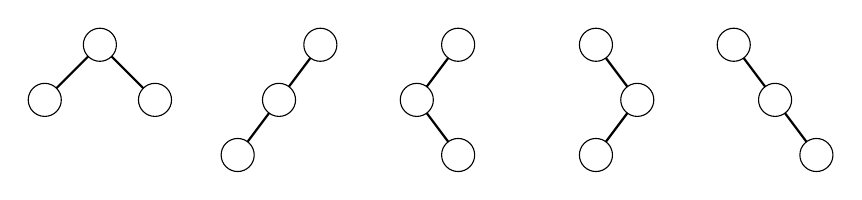
\begin{tikzpicture}[scale=0.7]
\path[draw,thick,-] (0,0) -- (-1,-1);
\path[draw,thick,-] (0,0) -- (1,-1);
\draw[fill=white] (0,0) circle (0.3);
\draw[fill=white] (-1,-1) circle (0.3);
\draw[fill=white] (1,-1) circle (0.3);

\path[draw,thick,-] (4,0) -- (4-0.75,-1) -- (4-1.5,-2);
\draw[fill=white] (4,0) circle (0.3);
\draw[fill=white] (4-0.75,-1) circle (0.3);
\draw[fill=white] (4-1.5,-2) circle (0.3);

\path[draw,thick,-] (6.5,0) -- (6.5-0.75,-1) -- (6.5-0,-2);
\draw[fill=white] (6.5,0) circle (0.3);
\draw[fill=white] (6.5-0.75,-1) circle (0.3);
\draw[fill=white] (6.5-0,-2) circle (0.3);

\path[draw,thick,-] (9,0) -- (9+0.75,-1) -- (9-0,-2);
\draw[fill=white] (9,0) circle (0.3);
\draw[fill=white] (9+0.75,-1) circle (0.3);
\draw[fill=white] (9-0,-2) circle (0.3);

\path[draw,thick,-] (11.5,0) -- (11.5+0.75,-1) -- (11.5+1.5,-2);
\draw[fill=white] (11.5,0) circle (0.3);
\draw[fill=white] (11.5+0.75,-1) circle (0.3);
\draw[fill=white] (11.5+1.5,-2) circle (0.3);
\end{tikzpicture}
\end{center}
y los árboles enraizados son
\begin{center}
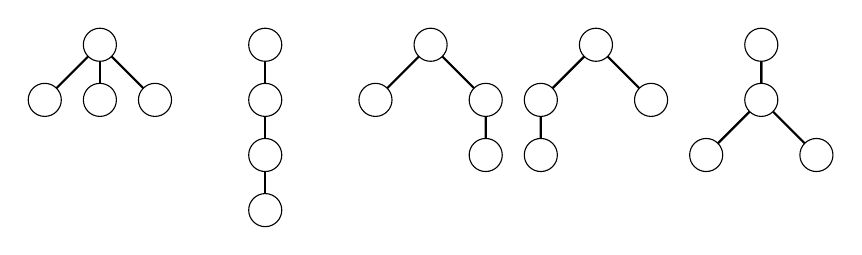
\begin{tikzpicture}[scale=0.7]
\path[draw,thick,-] (0,0) -- (-1,-1);
\path[draw,thick,-] (0,0) -- (0,-1);
\path[draw,thick,-] (0,0) -- (1,-1);
\draw[fill=white] (0,0) circle (0.3);
\draw[fill=white] (-1,-1) circle (0.3);
\draw[fill=white] (0,-1) circle (0.3);
\draw[fill=white] (1,-1) circle (0.3);

\path[draw,thick,-] (3,0) -- (3,-1) -- (3,-2) -- (3,-3);
\draw[fill=white] (3,0) circle (0.3);
\draw[fill=white] (3,-1) circle (0.3);
\draw[fill=white] (3,-2) circle (0.3);
\draw[fill=white] (3,-3) circle (0.3);

\path[draw,thick,-] (6+0,0) -- (6-1,-1);
\path[draw,thick,-] (6+0,0) -- (6+1,-1) -- (6+1,-2);
\draw[fill=white] (6+0,0) circle (0.3);
\draw[fill=white] (6-1,-1) circle (0.3);
\draw[fill=white] (6+1,-1) circle (0.3);
\draw[fill=white] (6+1,-2) circle (0.3);

\path[draw,thick,-] (9+0,0) -- (9+1,-1);
\path[draw,thick,-] (9+0,0) -- (9-1,-1) -- (9-1,-2);
\draw[fill=white] (9+0,0) circle (0.3);
\draw[fill=white] (9+1,-1) circle (0.3);
\draw[fill=white] (9-1,-1) circle (0.3);
\draw[fill=white] (9-1,-2) circle (0.3);

\path[draw,thick,-] (12+0,0) -- (12+0,-1) -- (12-1,-2);
\path[draw,thick,-] (12+0,0) -- (12+0,-1) -- (12+1,-2);
\draw[fill=white] (12+0,0) circle (0.3);
\draw[fill=white] (12+0,-1) circle (0.3);
\draw[fill=white] (12-1,-2) circle (0.3);
\draw[fill=white] (12+1,-2) circle (0.3);

\end{tikzpicture}
\end{center}

\section{Inclusión-exclusión}

\index{inclusión-exclusión}

\key{Inclusión-exclusión} es una técnica
que se puede usar para contar el tamaño
de una unión de conjuntos cuando se conocen los tamaños de
las intersecciones, y viceversa.
Un ejemplo simple de la técnica es la fórmula
\[ |A \cup B| = |A| + |B| - |A \cap B|,\]
donde $A$ y $B$ son conjuntos y $|X|$
denota el tamaño de $X$.
La fórmula se puede ilustrar como sigue:

\begin{center}
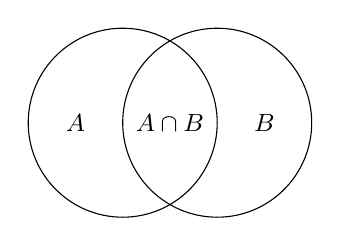
\begin{tikzpicture}[scale=0.8]

\draw (0,0) circle (1.5);
\draw (1.5,0) circle (1.5);

\node at (-0.75,0) {\small $A$};
\node at (2.25,0) {\small $B$};
\node at (0.75,0) {\small $A \cap B$};

\end{tikzpicture}
\end{center}

Nuestro objetivo es calcular
el tamaño de la unión $A \cup B$
que corresponde al área de la región
que pertenece a al menos un círculo.
La imagen muestra que podemos calcular
el área de $A \cup B$ sumando primero las
áreas de $A$ y $B$ y luego restando
el área de $A \cap B$.

La misma idea se puede aplicar cuando el número
de conjuntos es mayor.
Cuando hay tres conjuntos, la fórmula de inclusión-exclusión es
\[ |A \cup B \cup C| = |A| + |B| + |C| - |A \cap B|  - |A \cap C|  - |B \cap C| + |A \cap B \cap C| \]
y la imagen correspondiente es

\begin{center}
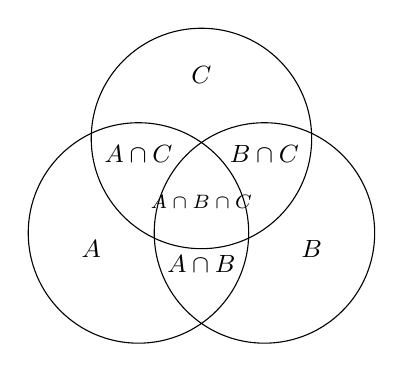
\begin{tikzpicture}[scale=0.8]

\draw (0,0) circle (1.75);
\draw (2,0) circle (1.75);
\draw (1,1.5) circle (1.75);

\node at (-0.75,-0.25) {\small $A$};
\node at (2.75,-0.25) {\small $B$};
\node at (1,2.5) {\small $C$};
\node at (1,-0.5) {\small $A \cap B$};
\node at (0,1.25) {\small $A \cap C$};
\node at (2,1.25) {\small $B \cap C$};
\node at (1,0.5) {\scriptsize $A \cap B \cap C$};

\end{tikzpicture}
\end{center}

En el caso general, el tamaño de la 
unión $X_1 \cup X_2 \cup \cdots \cup X_n$
se puede calcular recorriendo todas las posibles
intersecciones que contienen algunos de los conjuntos $X_1,X_2,\ldots,X_n$.
Si la intersección contiene un número impar de conjuntos,
su tamaño se agrega a la respuesta,
y de lo contrario su tamaño se resta de la respuesta.

Tenga en cuenta que hay fórmulas similares
para calcular
el tamaño de una intersección a partir de los tamaños de
uniones. Por ejemplo,
\[ |A \cap B| = |A| + |B| - |A \cup B|\]
y
\[ |A \cap B \cap C| = |A| + |B| + |C| - |A \cup B|  - |A \cup C|  - |B \cup C| + |A \cup B \cup C| .\]

\subsubsection{Desarreglos}

\index{desarreglo}

Como ejemplo, contemos el número de \key{desarreglos}
de elementos $\{1,2,\ldots,n\}$, es decir, permutaciones
donde ningún elemento permanece en su posición original.
Por ejemplo, cuando $n=3$, hay
dos desarreglos: $(2,3,1)$ y $(3,1,2)$.

Un enfoque para resolver el problema es usar
inclusión-exclusión.
Sea $X_k$ el conjunto de permutaciones
que contienen el elemento $k$ en la posición $k$.
Por ejemplo, cuando $n=3$, los conjuntos son los siguientes:
\[
\begin{array}{lcl}
X_1 & = & \{(1,2,3),(1,3,2)\} \\
X_2 & = & \{(1,2,3),(3,2,1)\} \\
X_3 & = & \{(1,2,3),(2,1,3)\} \\
\end{array}
\]
Usando estos conjuntos, el número de desarreglos es igual a
\[ n! - |X_1 \cup X_2 \cup \cdots \cup X_n|, \]
por lo que basta con calcular el tamaño de la unión.
Usando inclusión-exclusión, esto se reduce a
calcular tamaños de intersecciones que se pueden
hacer de manera eficiente.
Por ejemplo, cuando $n=3$, el tamaño de
$|X_1 \cup X_2 \cup X_3|$ es
\[
\begin{array}{lcl}
 & & |X_1| + |X_2| + |X_3| - |X_1 \cap X_2|  - |X_1 \cap X_3|  - |X_2 \cap X_3| + |X_1 \cap X_2 \cap X_3| \\
 & = & 2+2+2-1-1-1+1 \\
 & = & 4, \\
\end{array}
\]
por lo que el número de soluciones es $3!-4=2$.

Resulta que el problema también se puede resolver
sin usar inclusión-exclusión.
Sea $f(n)$ el número de desarreglos
para $\{1,2,\ldots,n\}$. Podemos usar la siguiente
fórmula recursiva:

\begin{equation*}
    f(n) = \begin{cases}
               0               & n = 1\\
               1               & n = 2\\
               (n-1)(f(n-2) + f(n-1)) & n>2 \\
           \end{cases}
\end{equation*}

La fórmula se puede derivar considerando
las posibilidades de cómo cambia el elemento 1
en el desarreglo.
Hay $n-1$ formas de elegir un elemento $x$
que reemplaza al elemento 1.
En cada una de estas elecciones, hay dos opciones:


\textit{Opción 1:} También reemplazamos el elemento $x$
con el elemento 1.
Después de esto, la tarea restante es construir
un desordenamiento de $n-2$ elementos.

\textit{Opción 2:} Reemplazamos el elemento $x$
con algún otro elemento que no sea 1.
Ahora tenemos que construir un desordenamiento
de $n-1$ elementos, porque no podemos reemplazar
el elemento $x$ con el elemento 1, y todos los demás
elementos deben ser cambiados.

\section{Lema de Burnside}

\index{Lema de Burnside}

\key{Lema de Burnside}
%\footnote{En realidad, Burnside no descubrió este lema; solo lo mencionó en su libro \cite{bur97}.}
se puede usar para contar
el número de combinaciones para que
solo se cuente un representante
para cada grupo de combinaciones simétricas.
El lema de Burnside establece que el número de
combinaciones es
\[\sum_{k=1}^n \frac{c(k)}{n},\]
donde hay $n$ maneras de cambiar la
posición de una combinación,
y hay $c(k)$ combinaciones que
permanecen sin cambios cuando se aplica la $k$-ésima forma.

Como ejemplo, calculemos el número de
collares de $n$ perlas,
donde cada perla tiene $m$ colores posibles.
Dos collares son simétricos si son
similares después de rotarlos.
Por ejemplo, el collar
\begin{center}
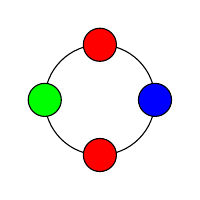
\begin{tikzpicture}[scale=0.7]
\draw[fill=white] (0,0) circle (1);
\draw[fill=red] (0,1) circle (0.3);
\draw[fill=blue] (1,0) circle (0.3);
\draw[fill=red] (0,-1) circle (0.3);
\draw[fill=green] (-1,0) circle (0.3);
\end{tikzpicture}
\end{center}
tiene los siguientes collares simétricos:
\begin{center}
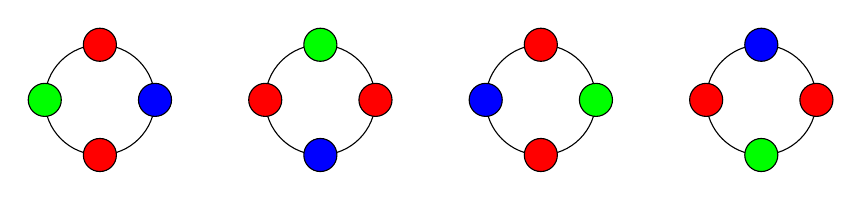
\begin{tikzpicture}[scale=0.7]
\draw[fill=white] (0,0) circle (1);
\draw[fill=red] (0,1) circle (0.3);
\draw[fill=blue] (1,0) circle (0.3);
\draw[fill=red] (0,-1) circle (0.3);
\draw[fill=green] (-1,0) circle (0.3);

\draw[fill=white] (4,0) circle (1);
\draw[fill=green] (4+0,1) circle (0.3);
\draw[fill=red] (4+1,0) circle (0.3);
\draw[fill=blue] (4+0,-1) circle (0.3);
\draw[fill=red] (4+-1,0) circle (0.3);

\draw[fill=white] (8,0) circle (1);
\draw[fill=red] (8+0,1) circle (0.3);
\draw[fill=green] (8+1,0) circle (0.3);
\draw[fill=red] (8+0,-1) circle (0.3);
\draw[fill=blue] (8+-1,0) circle (0.3);

\draw[fill=white] (12,0) circle (1);
\draw[fill=blue] (12+0,1) circle (0.3);
\draw[fill=red] (12+1,0) circle (0.3);
\draw[fill=green] (12+0,-1) circle (0.3);
\draw[fill=red] (12+-1,0) circle (0.3);
\end{tikzpicture}
\end{center}
Hay $n$ maneras de cambiar la posición
de un collar,
porque podemos rotarlo
$0,1,\ldots,n-1$ pasos en el sentido de las agujas del reloj.
Si el número de pasos es 0,
todos los $m^n$ collares permanecen iguales,
y si el número de pasos es 1,
solo los $m$ collares donde cada
perla tiene el mismo color permanecen iguales.

Más generalmente, cuando el número de pasos es $k$,
un total de
\[m^{\textrm{mcd}(k,n)}\]
collares permanecen iguales,
donde $\textrm{mcd}(k,n)$ es el máximo común
divisor de $k$ y $n$.
La razón de esto es que los bloques
de perlas de tamaño $\textrm{mcd}(k,n)$
se reemplazarán entre sí.
Por lo tanto, según el lema de Burnside,
el número de collares es
\[\sum_{i=0}^{n-1} \frac{m^{\textrm{mcd}(i,n)}}{n}. \]
Por ejemplo, el número de collares de longitud 4
con 3 colores es
\[\frac{3^4+3+3^2+3}{4} = 24. \]

\section{Fórmula de Cayley}

\index{Fórmula de Cayley}

\key{Fórmula de Cayley}
% \footnote{Si bien la fórmula lleva el nombre de A. Cayley,
% quien la estudió en 1889, fue descubierta antes por C. W. Borchardt en 1860.}
establece que
hay $n^{n-2}$ árboles etiquetados
que contienen $n$ nodos.
Los nodos están etiquetados $1,2,\ldots,n$,
y dos árboles son diferentes
si su estructura o
etiquetado es diferente.

\begin{samepage}
Por ejemplo, cuando $n=4$, el número de árboles etiquetados
es $4^{4-2}=16$:

\begin{center}
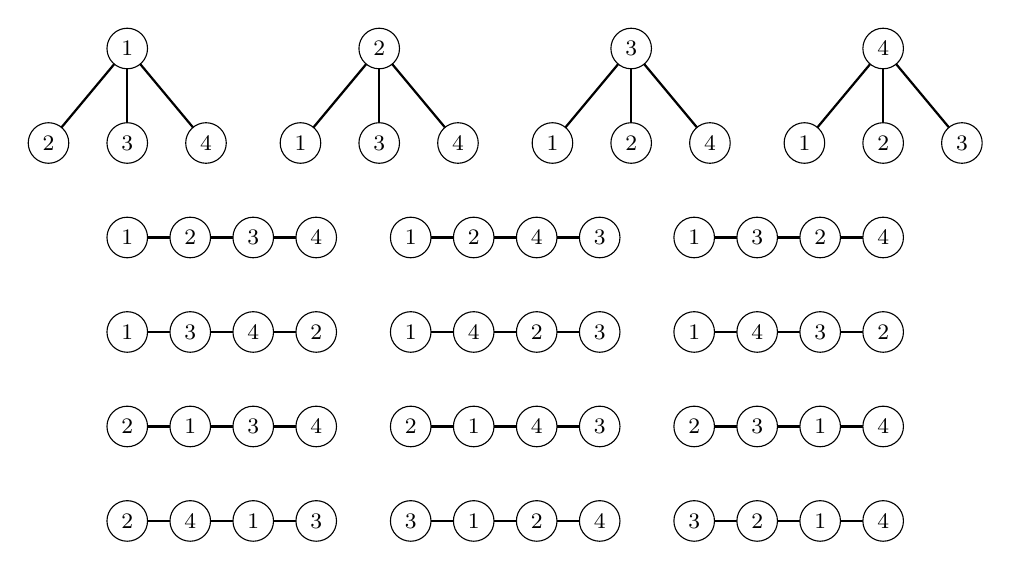
\begin{tikzpicture}[scale=0.8]
\footnotesize

\newcommand\puua[6]{
\path[draw,thick,-] (#1,#2) -- (#1-1.25,#2-1.5);
\path[draw,thick,-] (#1,#2) -- (#1,#2-1.5);
\path[draw,thick,-] (#1,#2) -- (#1+1.25,#2-1.5);
\node[draw, circle, fill=white] at (#1,#2) {#3};
\node[draw, circle, fill=white] at (#1-1.25,#2-1.5) {#4};
\node[draw, circle, fill=white] at (#1,#2-1.5) {#5};
\node[draw, circle, fill=white] at (#1+1.25,#2-1.5) {#6};
}
\newcommand\puub[6]{
\path[draw,thick,-] (#1,#2) -- (#1+1,#2);
\path[draw,thick,-] (#1+1,#2) -- (#1+2,#2);
\path[draw,thick,-] (#1+2,#2) -- (#1+3,#2);
\node[draw, circle, fill=white] at (#1,#2) {#3};
\node[draw, circle, fill=white] at (#1+1,#2) {#4};
\node[draw, circle, fill=white] at (#1+2,#2) {#5};
\node[draw, circle, fill=white] at (#1+3,#2) {#6};
}

\puua{0}{0}{1}{2}{3}{4}
\puua{4}{0}{2}{1}{3}{4}
\puua{8}{0}{3}{1}{2}{4}
\puua{12}{0}{4}{1}{2}{3}

\puub{0}{-3}{1}{2}{3}{4}
\puub{4.5}{-3}{1}{2}{4}{3}
\puub{9}{-3}{1}{3}{2}{4}
\puub{0}{-4.5}{1}{3}{4}{2}
\puub{4.5}{-4.5}{1}{4}{2}{3}
\puub{9}{-4.5}{1}{4}{3}{2}
\puub{0}{-6}{2}{1}{3}{4}
\puub{4.5}{-6}{2}{1}{4}{3}
\puub{9}{-6}{2}{3}{1}{4}
\puub{0}{-7.5}{2}{4}{1}{3}
\puub{4.5}{-7.5}{3}{1}{2}{4}
\puub{9}{-7.5}{3}{2}{1}{4}
\end{tikzpicture}
\end{center}
\end{samepage}

A continuación veremos cómo se puede
derivar la fórmula de Cayley utilizando códigos de Prüfer.

\subsubsection{Código de Prüfer}

\index{Código de Prüfer}

Un \key{código de Prüfer}
%\footnote{En 1918, H. Prüfer demostró el teorema de Cayley utilizando códigos de Prüfer \cite{pru18}.}
es una secuencia de
$n-2$ números que describe un árbol etiquetado.
El código se construye siguiendo un proceso
que elimina $n-2$ hojas del árbol.
En cada paso, se elimina la hoja con la etiqueta más pequeña,
y la etiqueta de su único vecino se agrega al código.

Por ejemplo, calculemos el código de Prüfer
del siguiente gráfico:
\begin{center}
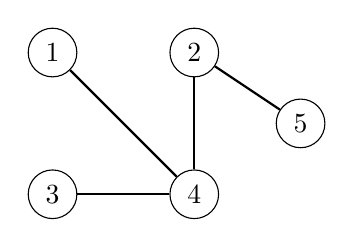
\begin{tikzpicture}[scale=0.9]
\node[draw, circle] (1) at (2,3) {$1$};
\node[draw, circle] (2) at (4,3) {$2$};
\node[draw, circle] (3) at (2,1) {$3$};
\node[draw, circle] (4) at (4,1) {$4$};
\node[draw, circle] (5) at (5.5,2) {$5$};

\path[draw,thick,-] (1) -- (4);
\path[draw,thick,-] (3) -- (4);
\path[draw,thick,-] (2) -- (4);
\path[draw,thick,-] (2) -- (5);
\end{tikzpicture}
\end{center}

Primero eliminamos el nodo 1 y agregamos el nodo 4 al código:
\begin{center}
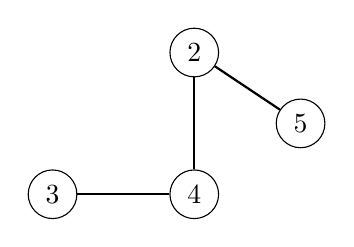
\begin{tikzpicture}[scale=0.9]
%\node[draw, circle] (1) at (2,3) {$1$};
\node[draw, circle] (2) at (4,3) {$2$};
\node[draw, circle] (3) at (2,1) {$3$};
\node[draw, circle] (4) at (4,1) {$4$};
\node[draw, circle] (5) at (5.5,2) {$5$};

%\path[draw,thick,-] (1) -- (4);
\path[draw,thick,-] (3) -- (4);
\path[draw,thick,-] (2) -- (4);
\path[draw,thick,-] (2) -- (5);
\end{tikzpicture}
\end{center}

Luego eliminamos el nodo 3 y agregamos el nodo 4 al código:
\begin{center}
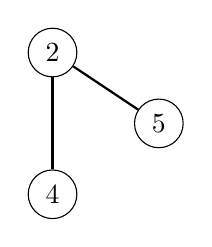
\begin{tikzpicture}[scale=0.9]
%\node[draw, circle] (1) at (2,3) {$1$};
\node[draw, circle] (2) at (4,3) {$2$};
%\node[draw, circle] (3) at (2,1) {$3$};
\node[draw, circle] (4) at (4,1) {$4$};
\node[draw, circle] (5) at (5.5,2) {$5$};

%\path[draw,thick,-] (1) -- (4);
%\path[draw,thick,-] (3) -- (4);
\path[draw,thick,-] (2) -- (4);
\path[draw,thick,-] (2) -- (5);
\end{tikzpicture}
\end{center}

Finalmente eliminamos el nodo 4 y agregamos el nodo 2 al código:
\begin{center}
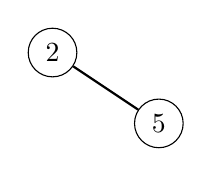
\begin{tikzpicture}[scale=0.9]
%\node[draw, circle] (1) at (2,3) {$1$};
\node[draw, circle] (2) at (4,3) {$2$};
%\node[draw, circle] (3) at (2,1) {$3$};
%\node[draw, circle] (4) at (4,1) {$4$};
\node[draw, circle] (5) at (5.5,2) {$5$};

%\path[draw,thick,-] (1) -- (4);
%\path[draw,thick,-] (3) -- (4);
%\path[draw,thick,-] (2) -- (4);
\path[draw,thick,-] (2) -- (5);
\end{tikzpicture}
\end{center}

Por lo tanto, el código de Prüfer del gráfico es $[4,4,2]$.

Podemos construir un código de Prüfer para cualquier árbol,
y lo que es más importante,
el árbol original se puede reconstruir
a partir de un código de Prüfer.
Por lo tanto, el número de árboles etiquetados
de $n$ nodos es igual a
$n^{n-2}$, el número de códigos de Prüfer
de tamaño $n$.
